% presentation.tex -- Zephyr RTOS: архитектура и устройство
\documentclass[12pt,aspectratio=169]{beamer}

% --- Кодировки и язык ---
\usepackage[T2A]{fontenc}
\usepackage[utf8]{inputenc}
\usepackage[russian]{babel}

% --- Тема ---
\usetheme{Madrid}
\usecolortheme{whale}

% --- Пакеты ---
\usepackage{graphicx}
\usepackage{listings}
\usepackage{xcolor}
\usepackage{amsmath}

% --- Настройка листингов ---
\lstset{
  basicstyle=\ttfamily\footnotesize,
  breaklines=true,
  frame=single,
  showstringspaces=false,
  keywordstyle=\color{blue},
  commentstyle=\color{gray},
  numbers=left,
  numberstyle=\tiny\color{gray},
  numbersep=5pt,
  tabsize=2,
  aboveskip=4pt,
  belowskip=4pt,
}

% --- Метаданные ---
\title{Zephyr RTOS: архитектура и устройство}
\date{2026}

\begin{document}

\frame{\titlepage}

% --- Содержание ---

\begin{frame}{Содержание}
\tableofcontents
\end{frame}

% --- 1. Зачем нужны RTOS? ---

\section{Зачем нужны RTOS?}

\begin{frame}{От суперцикла к RTOS}
\begin{columns}
\column{0.55\textwidth}
\begin{block}{Проблема суперцикла}
\begin{itemize}
  \item Один \texttt{while(1)} обрабатывает всё
  \item С ростом функциональности --- хаос
  \item Разные задачи требуют разного темпа
  \item Блокирующая операция (UART, TCP/IP) ломает тайминги
\end{itemize}
\end{block}
\column{0.45\textwidth}
\begin{block}{Эволюция}
\begin{enumerate}
  \item Суперцикл + временные метки
  \item Кооперативный планировщик
  \item Вытесняющий планировщик (RTOS)
\end{enumerate}
\end{block}
\end{columns}

\vspace{6pt}
\begin{alertblock}{Вывод}
RTOS нужна, когда сложность превышает возможности одного цикла:
TCP/IP + мотор + роборука + дисплей одновременно.
\end{alertblock}
\end{frame}

% ---

\begin{frame}{Кооперативный vs вытесняющий планировщик}
\begin{block}{Кооперативный}
\begin{itemize}
  \item Задача сама отдаёт управление
  \item Одна медленная задача блокирует все остальные
  \item Прост в реализации, но не масштабируется
\end{itemize}
\end{block}

\pause

\begin{block}{Вытесняющий (preemptive) --- основа RTOS}
\begin{itemize}
  \item Аппаратный таймер (например, 1\,мс) вызывает прерывание
  \item Планировщик может \textbf{принудительно} переключить задачу
  \item Сохраняется/восстанавливается контекст (регистры, стек)
  \item Медленная задача не мешает критичным по времени
\end{itemize}
\end{block}
\end{frame}

% --- 2. Отличия Zephyr ---

\section{Отличия Zephyr от других RTOS}

\begin{frame}{Zephyr: что выделяет его среди RTOS}
\begin{enumerate}
  \item \textbf{Linux Foundation} --- поддержка крупнейшего open-source фонда
  \item \textbf{Родство с Linux} --- Kconfig, DeviceTree, общие концепции
  \item \textbf{Гибкая конфигурация} --- Kconfig позволяет включить только нужное
  \item \textbf{Широкая поддержка архитектур}
\end{enumerate}

\pause
\vspace{4pt}
\begin{block}{Поддерживаемые архитектуры}
\footnotesize
ARCv2/ARCv3 \;|\; ARMv6-M/v7-M/v8-M (Cortex-M) \;|\;
ARMv7-A/v8-A (Cortex-A, 32/64-bit) \;|\;
ARMv7-R/v8-R (Cortex-R) \;|\;
Intel x86 (32/64-bit) \;|\; MIPS32 \;|\;
OpenRISC \;|\; Renesas RX \;|\;
\textbf{RISC-V (32/64-bit)} \;|\; SPARC V8 \;|\; Tensilica Xtensa
\end{block}
\end{frame}

% --- 3. Архитектура Zephyr ---

\section{Архитектура Zephyr}

\begin{frame}{Системная архитектура Zephyr}
\begin{center}
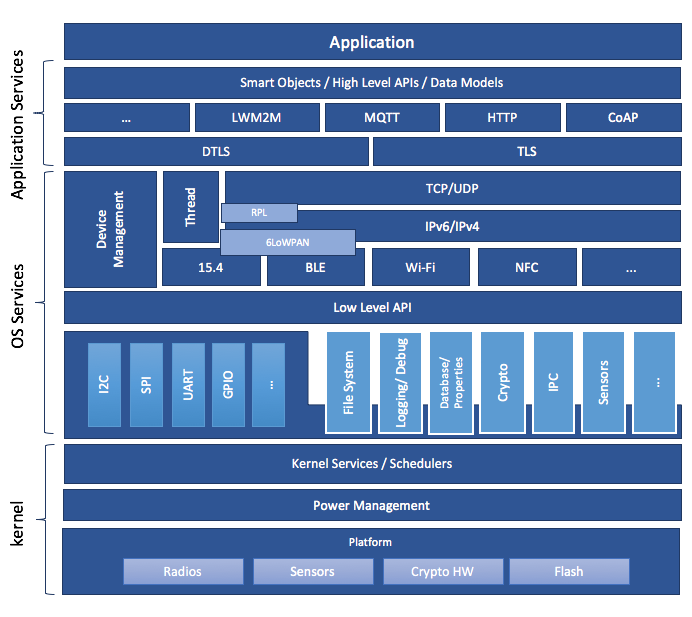
\includegraphics[width=0.82\textwidth]{security-zephyr-system-architecture.png}
\end{center}
\end{frame}

% ---

\begin{frame}[fragile]{Структура проекта Zephyr}
\begin{columns}
\column{0.5\textwidth}
\begin{block}{Ключевые файлы}
\begin{itemize}
  \item \texttt{CMakeLists.txt} --- сборка
  \item \texttt{prj.conf} --- конфигурация (Kconfig)
  \item \texttt{src/} --- исходный код
  \item \texttt{build/} --- артефакты сборки
\end{itemize}
\end{block}
\column{0.5\textwidth}
\begin{block}{Пример prj.conf}
\begin{lstlisting}[language={}]
CONFIG_PRINTK=y
CONFIG_SERIAL=y
CONFIG_HEAP_MEM_POOL_SIZE=256
\end{lstlisting}
\end{block}
\end{columns}
\end{frame}

% --- 4. Ядро Zephyr ---

\section{Ядро Zephyr}

\begin{frame}{Ядро Zephyr: основа каждого приложения}
\begin{block}{Характеристики}
\begin{itemize}
  \item Малозатратная многопоточная среда
  \item Минимальный footprint --- \textbf{от 2 КБ}
  \item Для сложных систем --- 50--900 КБ (BLE, Wi-Fi, сложная многопоточность)
  \item Модульная архитектура: включается только нужное
\end{itemize}
\end{block}

\vspace{4pt}
\begin{block}{Сервисы ядра}
Планировщик \;|\; Управление потоками \;|\;
Синхронизация (семафоры, мьютексы, очереди) \;|\;
Управление памятью \;|\; Таймеры \;|\; Обработка прерываний
\end{block}
\end{frame}

% --- 5. Потоки ---

\section{Потоки}

\begin{frame}{Поток (Thread) --- что это?}
\begin{block}{Определение}
Поток --- изолированный экземпляр, выполняющий некоторую задачу.
RTOS создаёт иллюзию одновременного выполнения на одном CPU
путём переключения контекста.
\end{block}

\pause
\begin{block}{Составные части потока}
\begin{description}
  \item[Стек] область памяти под стек потока. \texttt{\#define STACKSIZE 1024}
  \item[Блок управления] \texttt{struct k\_thread} --- метаданные потока
  \item[Точка входа] функция, вызываемая при запуске
  \item[Приоритет] политика планирования
  \item[Режим] супервизор (по умолчанию) или пользователь
\end{description}
\end{block}
\end{frame}

% ---

\begin{frame}[fragile]{Пример создания потока}
\begin{lstlisting}[language=C]
#include <zephyr/kernel.h>

#define STACKSIZE 1024
K_THREAD_STACK_DEFINE(thread_a_stack, STACKSIZE);
static struct k_thread thread_a_data;

void thread_a_entry(void *d1, void *d2, void *d3)
{
    ARG_UNUSED(d1); ARG_UNUSED(d2); ARG_UNUSED(d3);
    hello_loop(__func__, &thread_a_sem, &thread_b_sem);
}

void main(void)
{
    k_thread_create(&thread_a_data, thread_a_stack,
        K_THREAD_STACK_SIZEOF(thread_a_stack),
        thread_a_entry, NULL, NULL, NULL,
        MY_PRIORITY, 0, K_NO_WAIT);
}
\end{lstlisting}
\end{frame}

% --- 6. Планировщик ---

\section{Планировщик}

\begin{frame}{Планировщик (Scheduler)}
\begin{block}{Принцип работы}
Приоритетный планировщик: потоки разделяют процессорное время.
Переключение происходит в \textbf{точках изменения расписания}:
\end{block}

\begin{columns}
\column{0.5\textwidth}
\begin{itemize}
  \item \texttt{k\_sem\_take()} / \texttt{k\_sleep()} --- поток засыпает
  \item \texttt{k\_sem\_give()} / \texttt{k\_thread\_start()} --- пробуждение
  \item Возврат из ISR
  \item \texttt{k\_yield()} --- явная передача управления
\end{itemize}
\column{0.5\textwidth}
\begin{center}
\textbf{Сохранение контекста}

\vspace{6pt}
При переключении ядро сохраняет:
\begin{itemize}
  \item Регистры CPU
  \item Указатель стека
  \item Счётчик команд
\end{itemize}
\vspace{4pt}
При возобновлении --- восстанавливает.
\end{center}
\end{columns}
\end{frame}

% ---

\begin{frame}{Состояния потоков}
\begin{center}
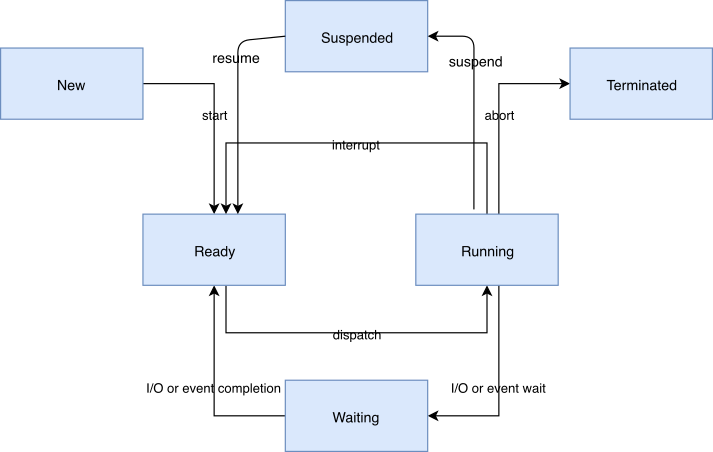
\includegraphics[width=0.75\textwidth]{thread-states.png}
\end{center}
\end{frame}

% ---

\begin{frame}{Тайм-слайсинг и сон}
\begin{block}{Тайм-слайсинг}
\begin{itemize}
  \item Время делится на \textbf{временные интервалы} (такты)
  \item В конце интервала --- неявный \texttt{k\_yield()} для вытесняемых потоков
  \item Не гарантирует равного времени, но гарантирует: поток не выполняется дольше одного интервала без необходимости
\end{itemize}
\end{block}

\pause
\begin{block}{Управление выполнением}
\footnotesize
\begin{description}
  \item[\texttt{k\_sleep()}] отложить обработку на N мс. CPU освобождается
  \item[\texttt{k\_wakeup()}] разбудить спящий поток преждевременно
  \item[\texttt{k\_sched\_lock()}] временно запретить вытеснение (критическая секция)
  \item[\texttt{k\_cpu\_idle()}] перевести процессор в режим ожидания (c\_idle.c)
  \item[\texttt{k\_yield()}] явно уступить CPU
\end{description}
\end{block}
\end{frame}

% --- 7. Управление памятью ---

\section{Управление памятью}

\begin{frame}{Типы памяти во встраиваемых системах}
\begin{columns}
\column{0.33\textwidth}
\begin{block}{SRAM}
\begin{itemize}
  \item Рабочая память (runtime)
  \item Минимальная задержка
  \item Куча, стеки, глобальные переменные
  \item КБ--МБ
\end{itemize}
\end{block}
\column{0.33\textwidth}
\begin{block}{Flash}
\begin{itemize}
  \item Энергонезависимая
  \item Код + константы
  \item Execute-in-place (XIP)
  \item Медленная запись
\end{itemize}
\end{block}
\column{0.33\textwidth}
\begin{block}{Cache}
\begin{itemize}
  \item Буфер CPU--память
  \item Кэш команд и данных
  \item Критичен для производительности
\end{itemize}
\end{block}
\end{columns}
\end{frame}

% ---

\begin{frame}{Регионы памяти Zephyr}
\begin{center}
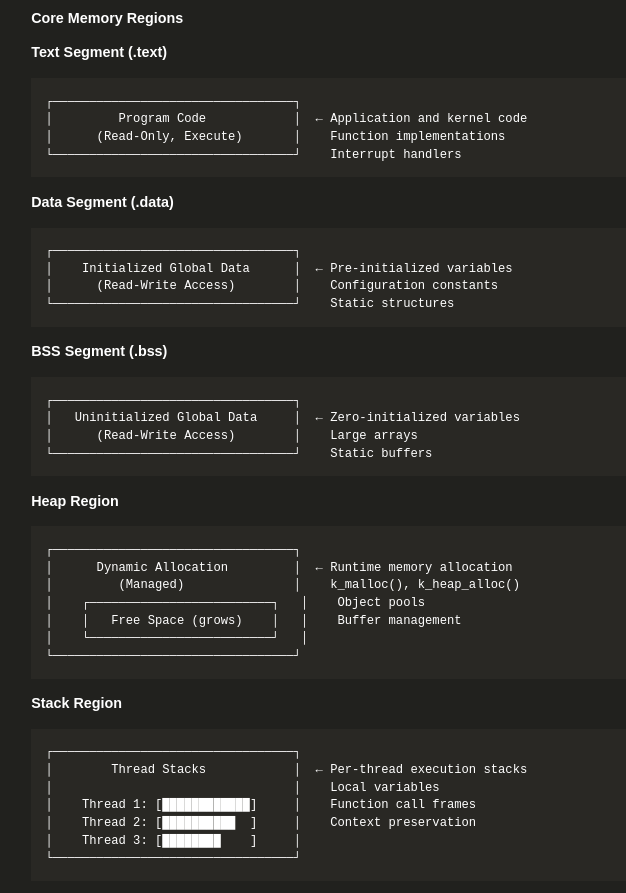
\includegraphics[width=0.55\textwidth]{memory_regions.png}
\end{center}
\begin{block}{Области}
Zephyr чётко разделяет память на регионы:
Code (Flash) \;|\; Data \;|\; BSS \;|\;
Heap \;|\; Thread Stacks \;|\;
Kernel objects \;|\; Device MMIO
\end{block}
\end{frame}

% ---

\begin{frame}[fragile]{Статическое vs динамическое выделение}
\begin{columns}
\column{0.5\textwidth}
\begin{block}{Статическое}
\begin{itemize}
  \item Выделение на этапе компиляции
  \item Нулевые накладные расходы
  \item Детерминированное поведение
  \item Нет риска фрагментации
  \item Идеально для систем реального времени
\end{itemize}
\end{block}
\column{0.5\textwidth}
\begin{block}{Динамическое}
\begin{itemize}
  \item Гибкость во время выполнения
  \item Эффективное использование памяти
  \item Структуры переменного размера
  \item Риск: фрагментация, отказ выделения
  \item Накладные расходы runtime
\end{itemize}
\end{block}
\end{columns}

\vspace{6pt}
\begin{lstlisting}[language=C, basicstyle=\ttfamily\scriptsize]
// Static allocation
static uint8_t sensor_buffer[1024];
K_THREAD_STACK_DEFINE(sensor_stack, 2048);

// Dynamic allocation
void *buf = k_heap_alloc(&app_heap, 256, K_FOREVER);
\end{lstlisting}
\end{frame}

% ---

\begin{frame}[fragile]{API кучи Zephyr}
\begin{block}{Статическая куча}
\begin{lstlisting}[language=C, basicstyle=\ttfamily\scriptsize]
K_HEAP_DEFINE(app_heap, 8192); // at compile time
\end{lstlisting}
\end{block}

\pause
\begin{block}{Динамическая куча (runtime)}
\begin{lstlisting}[language=C, basicstyle=\ttfamily\scriptsize]
static uint8_t heap_mem[8192];
static struct k_heap custom_heap;
k_heap_init(&custom_heap, heap_mem, sizeof(heap_mem));
\end{lstlisting}
\end{block}

\pause
\begin{block}{Функции}
\begin{lstlisting}[language=C, basicstyle=\ttfamily\scriptsize]
void *k_heap_alloc(struct k_heap *h, size_t bytes, k_timeout_t t);
void *k_heap_calloc(struct k_heap *h, size_t n, size_t sz, k_timeout_t t);
void  k_heap_free(struct k_heap *h, void *mem);
// stdlib-compatible: malloc(), calloc(), realloc(), free()
\end{lstlisting}
\end{block}
\end{frame}

% ---

\begin{frame}[fragile]{Пример работы с кучей}
\begin{lstlisting}[language={}, basicstyle=\ttfamily\scriptsize]
*** Booting Zephyr OS build v4.3.0 ***
System heap sample

allocated 0,   free 196, max allocated 0,   heap size 256
allocated 156, free 36,  max allocated 156, heap size 256
allocated 100, free 92,  max allocated 156, heap size 256
allocated 0,   free 196, max allocated 156, heap size 256

1 static heap(s) allocated:
  0 - addr 0x10000034  alloc 12, free 180, max alloc 12, size 256
3 heap(s) allocated (including static):
  0 - addr 0x10000034  alloc 12, free 180, max alloc 12, size 256
  1 - addr 0x1000036c  alloc 0,  free 60676, max alloc 0, size 256
  2 - addr 0x10000250  alloc 0,  free 196, max alloc 156, size 256
\end{lstlisting}
\end{frame}

% --- 8. Заключение ---

\section{Заключение}

\begin{frame}{Итоги}
\begin{block}{Zephyr RTOS предоставляет}
\begin{itemize}
  \item Вытесняющий приоритетный планировщик
  \item Изолированные потоки с сохранением контекста
  \item Примитивы синхронизации: семафоры, мьютексы, очереди
  \item Гибкое управление памятью: статика + динамика
  \item Модульное ядро (от 2 КБ)
  \item Поддержку 10+ архитектур, включая RISC-V
  \item Стек протоколов: TCP/IP, Bluetooth, USB
\end{itemize}
\end{block}

\vspace{4pt}
\begin{center}
\end{center}
\end{frame}

\end{document}
